\lecture{3}{9 Sep. 15:30}{}
Actually we have an alternitive prove:
\begin{proof}[proof by direct computation]
    \vphantom{text}
\begin{itemize}
    \item Q1: Who's the opponent for the \(1\)-st player? There are \(5\) choices. 
    \item Q2: Who plays the next lowest numbered player? There are \(3\) choices.   
\end{itemize}
The left \(2\) players are the opponents to each other. Hence, there are \(3 \times 5 = 15\)possible pairings.  
\end{proof}

More generally, if we have \(n = 2k\) players to pair up, then the first proof gives there are 
\[
    \frac{\binom{n}{2} \binom{n-2}{2}\dots \binom{2}{2}}{\left( \frac{n}{2} \right)!}
\]possible pairings, while the second proof gives that there are 
\[
    (n-1) \cdot (n - 3) \cdot (n-5) \dots \coloneqq (n-1)!! \neq \left( (n-1)! \right)!  .
\]

By this, we know these two numbers must be equal, or more rigorously, we can write 
\[
  \frac{\binom{n}{2} \binom{n-2}{2}\dots \binom{2}{2}}{\left( \frac{n}{2} \right)!} = 2^n \cdot \frac{\frac{n(n-1)}{2} \frac{(n-2)(n-3)}{2} \dots }{n(n-2)(n-4)\dots 2}  = (n-1) \cdot (n-3) \cdot \dots 
\]

\begin{eg}
    How mant shortest routes on the grid are there from \((0, 0)\) to \((n, m)\)?  
\end{eg}

\begin{figure}[H]
    \centering
    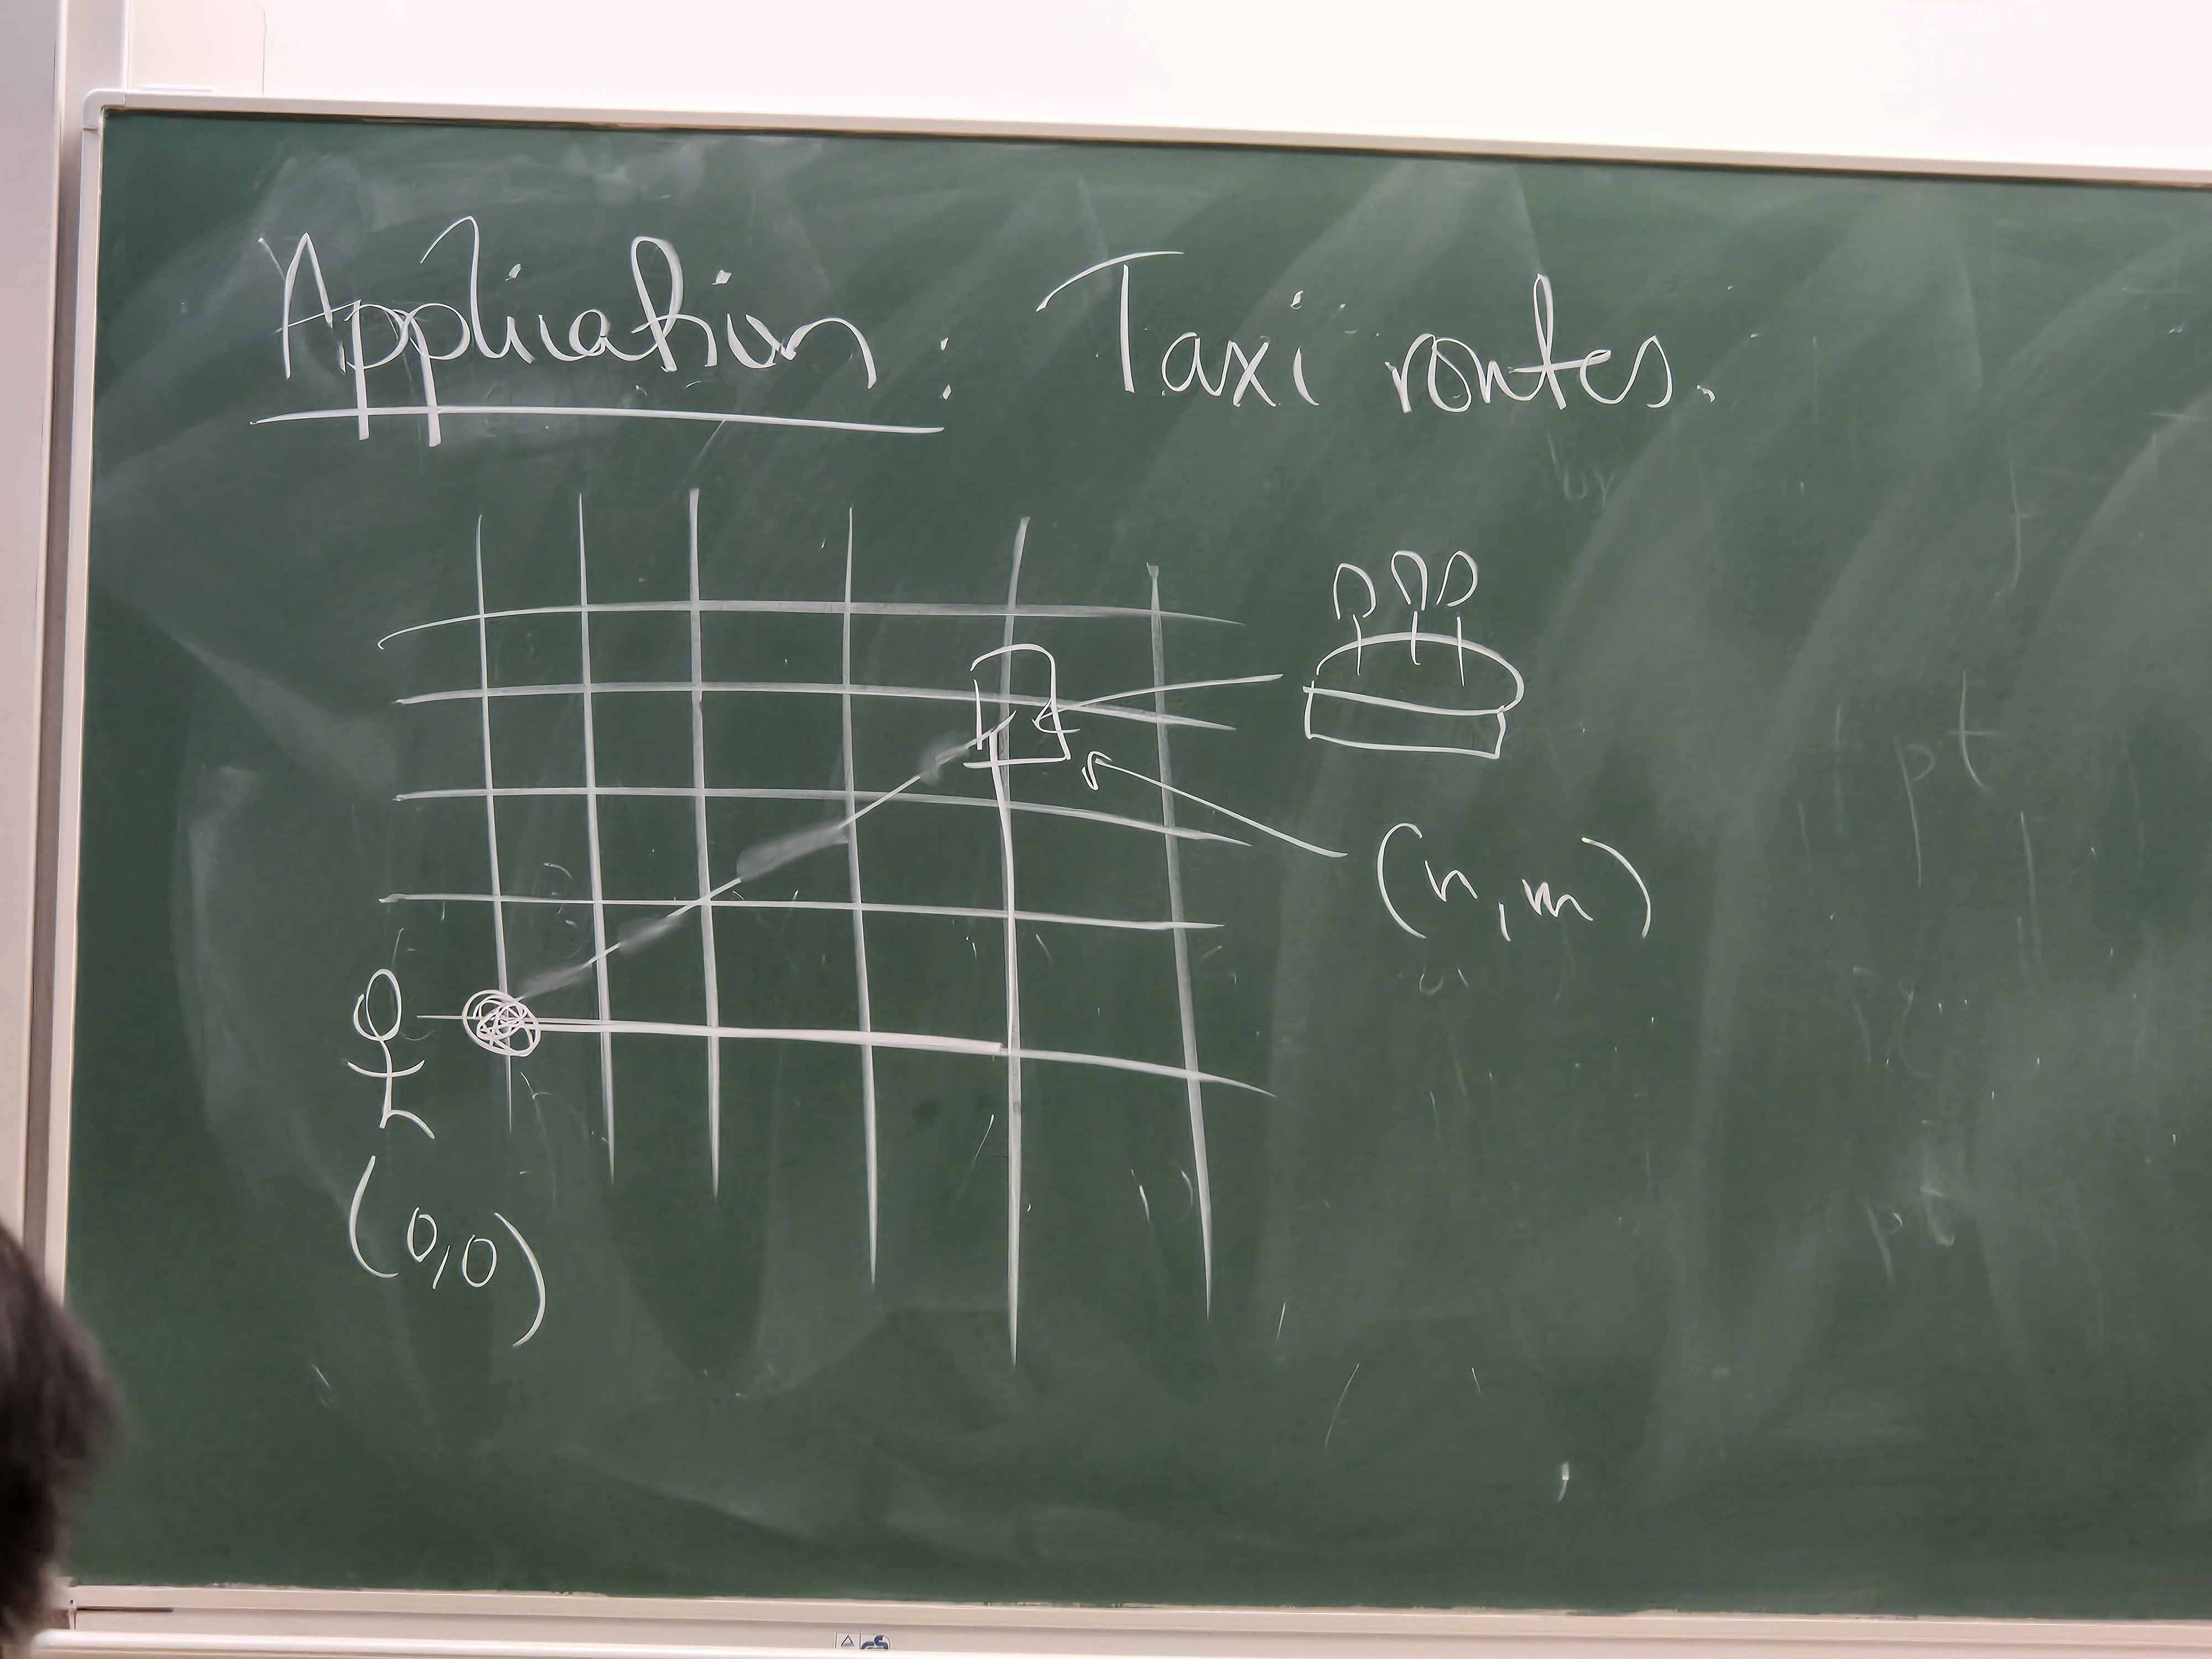
\includegraphics[width=0.8\textwidth]{./Figures/20250909_155011.jpg}
    \caption{Taxi routes}
    \label{fig:taxi routes}
\end{figure}
\begin{explanation}
    Shortest route is of length \(n + m\),\(m\) up-steps and \(n\) right-steps. We can think of a shortest route to be a binary string of length \(n + m\) with \(n\) \(1\)s and \(m\) \(0\)s, so we want to count how many such binary strings are there. Choose \(n\) of them to be \(1\)s, while the other are \(0\)s.  Hence, there are \(\binom{n+m}{n}\) possibilities.     
\end{explanation}

\section{Binomial Theorem}
\begin{theorem}[Binomial Theorem] \label{thm: binomial theorem}
    For any \(n \in \mathbb{N} \cup \left\{ 0 \right\} \), and \(x, y \in \mathbb{R} \), we have 
    \[
        (x + y)^n = \sum_{k=0}^n \binom{n}{k} x^k y^{n-k} 
    \]  
\end{theorem}
\begin{eg}
    \((x+y)^0 = 1 = \sum_{k=0} ^0 x^k y^{0-k}\). 
\end{eg}

\begin{eg}
    \((x + y)^1 = x+y\), while 
    \[
        \sum_{k=0}^1 \binom{1}{k}x^k y^{1-k} = \binom{1}{0}x^0 y^1 + \binom{1}{1} x^1 y^0 = y + x . 
    \] 
\end{eg}

\begin{proof}[proof of binomial theorem]
\begin{align*}
    (x + y)^n = \underbrace{(x+y)(x+y)(x+y) \dots (x+y)}_{n \text{ factors}}
\end{align*}
From each factor, we pick a term \(x\) or \(y\), multuply chosen factors together. If we choose \(k\) \(x\)'s, then we must choose \(n - k\) \(y\)'s, so the monomial is \(x^k y^{n-k}\), where the coefficient of \(x^k y^{n-k}\) is the number of ways of choosing \(k\) \(x\)'s. Also, the possible monomials are \(x^k y^{n-k}\) for \(k=0,1,2,\dots ,n\). Hence, we have 
\[
    (x + y)^n = \sum_{k=0}^n \binom{n}{k} x^k y^{n-k}. 
\]            
\end{proof}

We can use this formula to derive identities for the binomial coefficients, by plugging in values for \(x\) and \(y\). 

\begin{eg}
    \(x = 1, y = 1\). 
\end{eg}
\begin{explanation}
    \[
        2^n = (x + y)^n = \sum_{k=0}^n \binom{n}{k}x^k y^{n-k} = \sum_{k=0}^n \binom{n}{k}. 
    \]
\end{explanation}

\begin{eg}
    \(y = -1, x = 1\).  
\end{eg}
\begin{explanation}
    \begin{align*}
        (x + y) ^n &= (-1 + 1)^n = 0^n = \begin{dcases}
           1 , &\text{ if } n=0 ;\\
           0 , &\text{ if } n \ge 1.
        \end{dcases} \\
        (x+y)^n &= \sum_{k=0}^n \binom{n}{k} x^k y^{n-k} = \sum_{k=0}^n \binom{n}{k} (-1)^k = \sum_{2 \mid k} \binom{n}{k} - \sum_{2 \nmid k} \binom{n}{k}    
    \end{align*}
\end{explanation}

\begin{corollary}
    \[
        \sum_{2 \mid k} \binom{n}{k} = \sum_{2 \nmid k} \binom{n}{k}  
    \]
\end{corollary}
\begin{figure}[H]
    \centering
    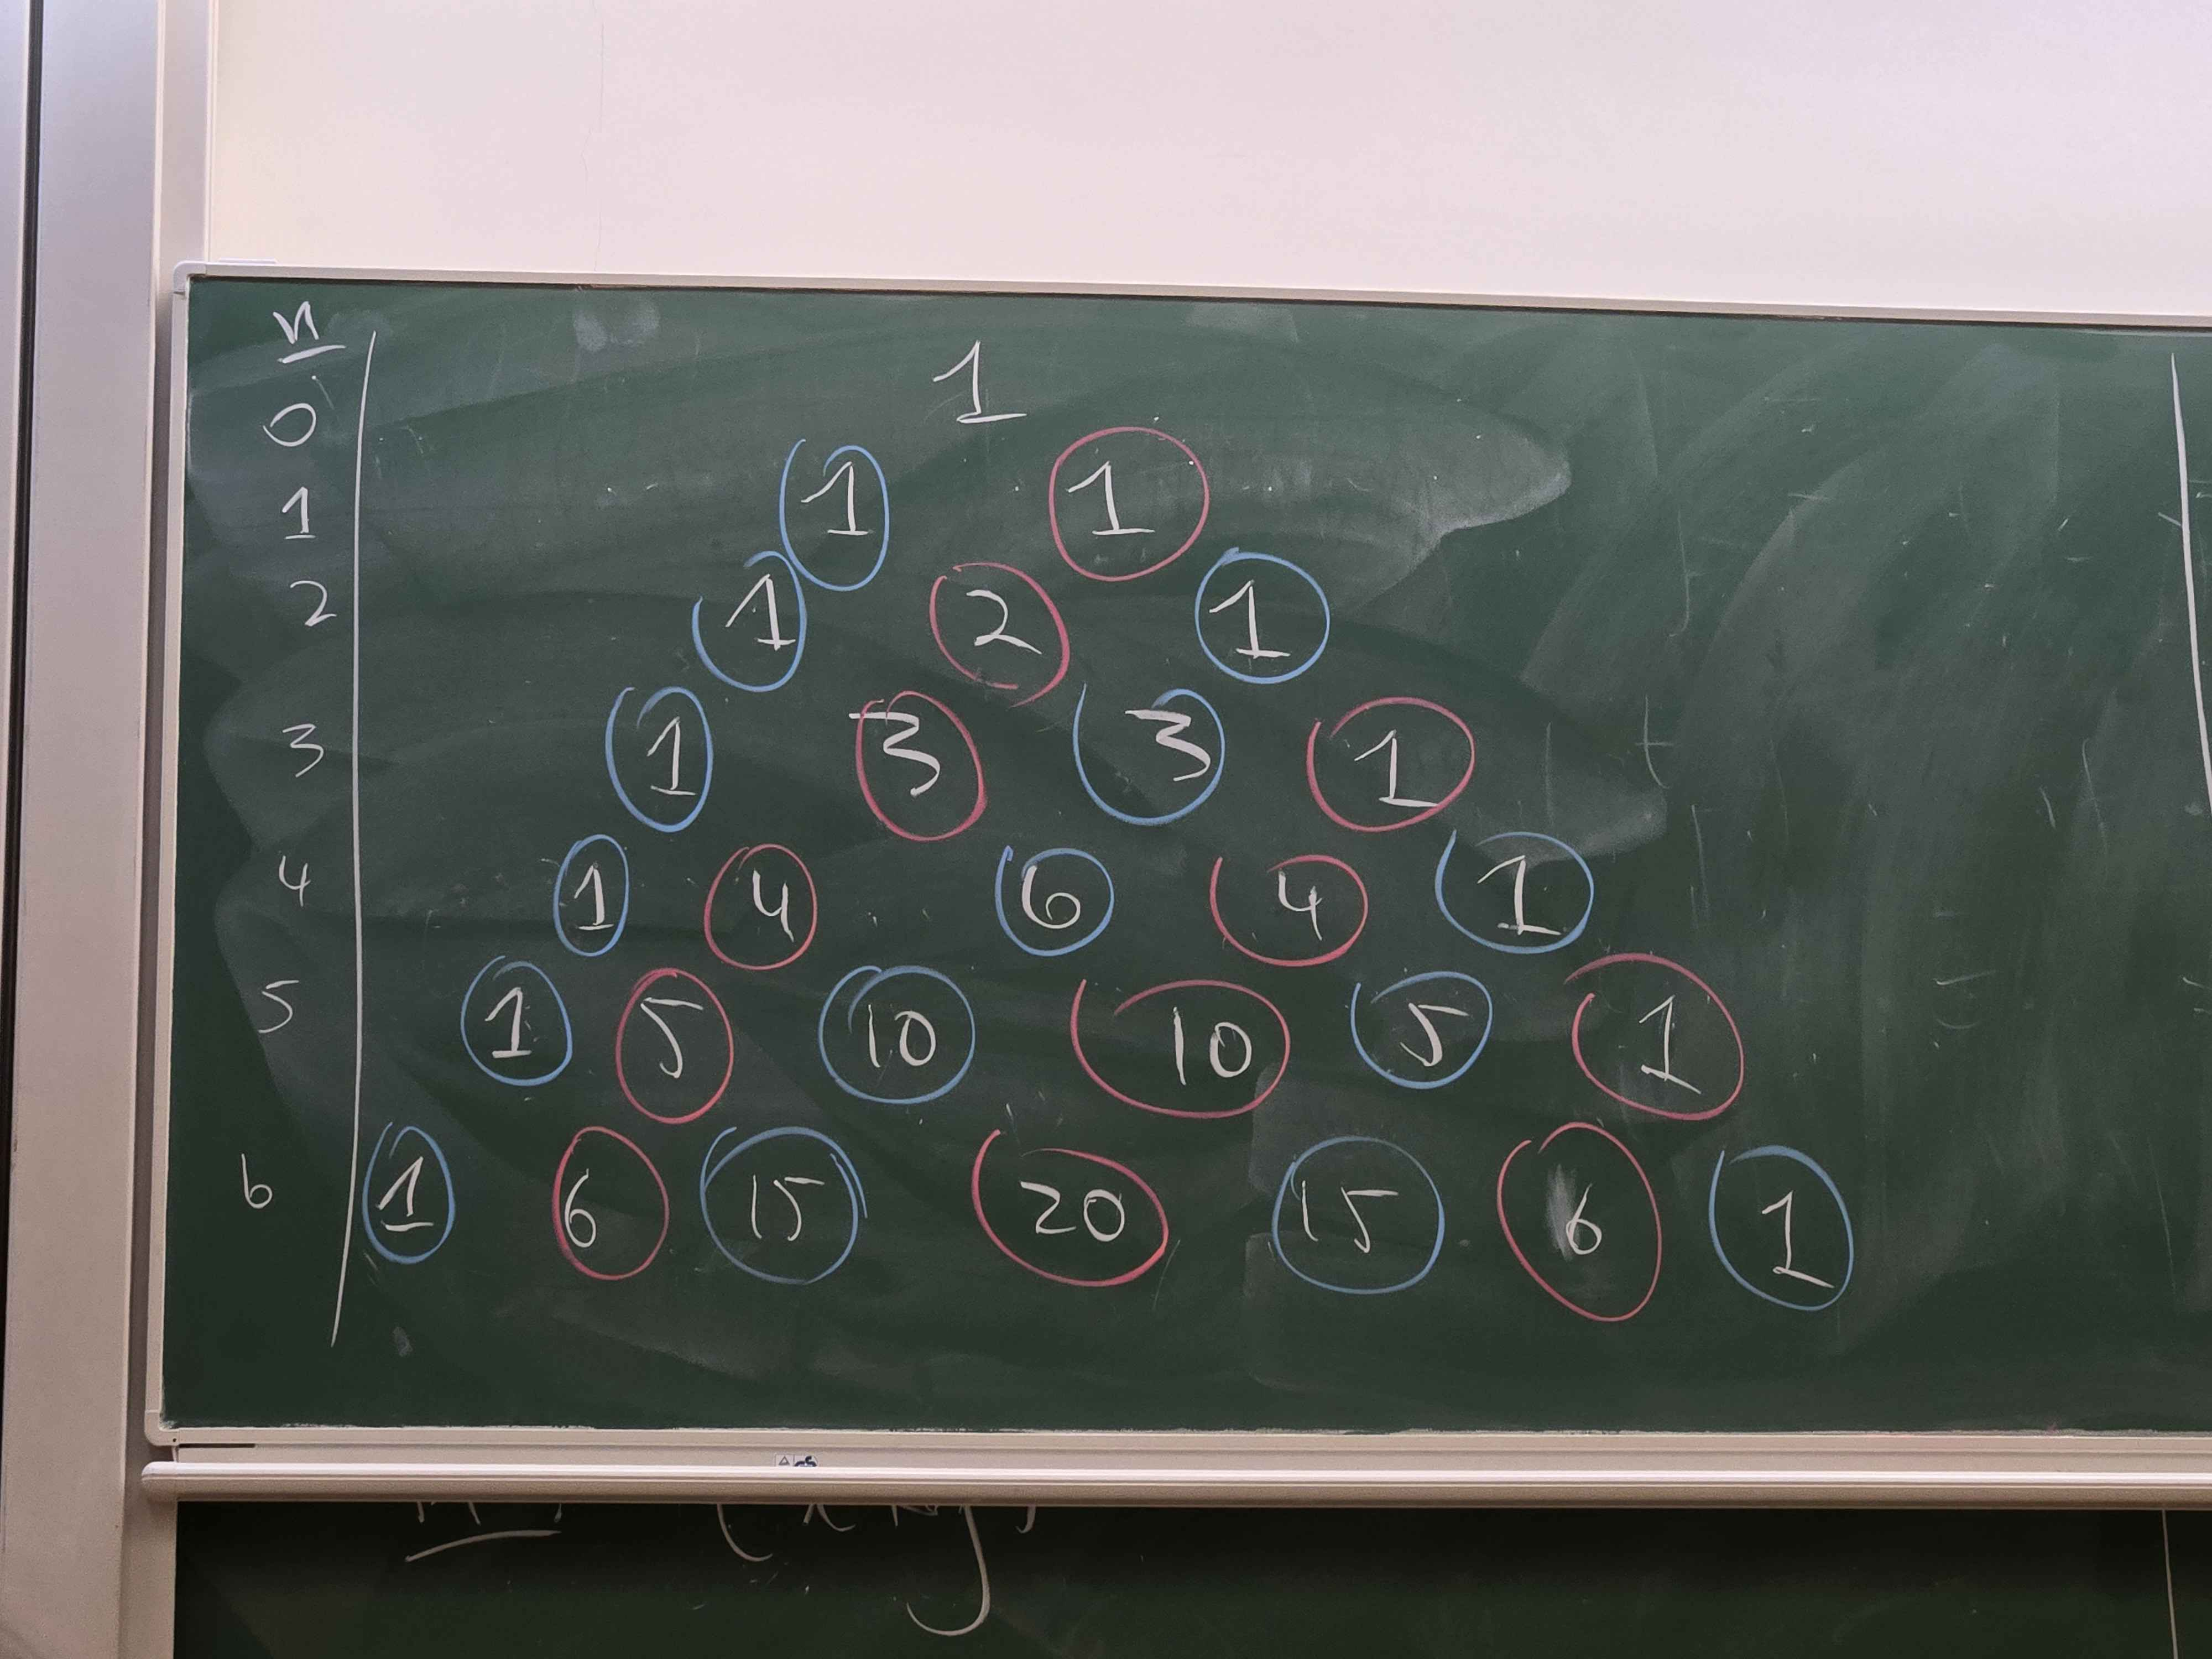
\includegraphics[width=0.8\textwidth]{./Figures/20250909_161713.jpg}
    \caption{The sum of even terms is equal to the sum of odd terms.}
    \label{fig:binomial term even odd relation}
\end{figure}

\begin{theorem}
    \(\forall n \ge k\), we have 
    \[
        \binom{n}{k} = \binom{n}{n-k}.
    \] 
\end{theorem}
\begin{proof}
    \[
        \binom{n}{k}=\frac{n!}{k!(n-k)!} = \frac{n!}{(n-k)!k!} = \frac{n!}{(n - (n-k))!}=\binom{n}{n-k}.
    \]
    \begin{remark}
        Choosing a subset of \(k\) elements from \(n\) is equivalent to choose \(n-k\) elements to discard, and we can build a bijection between these two methods.    
    \end{remark}
\end{proof}

For \(n\) even. 

Consider the bijection 
\[
    S \mapsto S \triangle \left\{ n \right\} = \begin{dcases}
       S - \left\{ n \right\}  , &\text{ if } n \in S  ;\\
       S \cup \left\{ n \right\}  , &\text{ if } n \notin S.
    \end{dcases} 
\]
Hence, 
\[
    \vert S \triangle \left\{ n \right\}  \vert \in \left\{ \vert S \vert - 1, \vert S \vert + 1   \right\},   
\] so if \(\vert S \vert \) is odd, then \(S \triangle \left\{ n \right\} \) is even, and vice versa. We know this is a bijection (self-inverse), so we have odd-sized sets to even-sized set. Hence, \(\sum_{2 \mid k} \binom{n}{k} = \sum_{2 \nmid k} \binom{n}{k}  \). 

\begin{eg}
    \(x=2, y=1\). 
\end{eg}
\begin{explanation}
    \begin{align*}
       (2 + 1)^n = 3^n = \sum_{k=0}^n \binom{n}{k} 2^k 
    \end{align*}
    Counting partitions \([n] = A \cupdot B \cupdot C\), each element has a choice of \(3\) sets to go into. Hence, the product rule says there are \(3^n\) partitions, while RHS uses sum rule bases on \(k = \vert A \cup B \vert \).    
\end{explanation}

\section{Divisor Function}
\begin{definition}[Divisor Functions] \label{def: divisor func}
    Given a natural number \(n \in \mathbb{N} \), let \(d(n)\) count the number of divisors of \(n\).   
\end{definition}

\begin{eg}
    \begin{align*}
        d(1) &= 1 = \vert \left\{ 1 \right\}  \vert \\
        d(2) &= 2 = \vert \left\{ 1,2 \right\}  \vert \\
        d(3) &= 2 = \vert \left\{ 1, 3 \right\}  \vert   \\
        d(4) &= 3 = \vert \left\{ 1, 2, 4 \right\}  \vert \\
        d(5) &= 2 = \vert \left\{ 1, 5 \right\}  \vert.  
    \end{align*}
\end{eg}

\begin{corollary}
    \(d(n) = 2\) if and only if \(n\) is a prime.  
\end{corollary}

Now we want to compute the average value of \(d(n)\). 

\begin{definition}
    \[
        \overline{d}(n) = \frac{\sum_{i=1}^n d(i)}{n}.  
    \]
\end{definition}

We can use double-counting. First, notice that 
\[
    d(i) = \sum_{\substack{j \in [i] \\ j \mid i}} 1. 
\]
Hence, 
\[
    \sum_{i=1}^n d(i) = \sum_{i=1}^n \sum_{\substack{j \in [i] \\ j \mid i}} 1. 
\]

We can exchange the order of summation: 
\[
    n \overline{d}(n) = \sum_{i=1}^n d(i) = \sum_{i=1}^n \sum_{j: j \mid i} 1 = \sum_{j=1}^n \sum_{\substack{i \in [n] \\ j \mid i}} 1.
\]

For fixed \(j\), we know 
\[
    \sum_{\substack{i \in [n] \\ j \mid i}} 1 = \left\lfloor \frac{n}{j} \right\rfloor.
\] 

Hence, we have 
\[
    n \overline{d}(n) = \sum_{j=1}^n \left\lfloor \frac{n}{j} \right\rfloor,
\] which is equivalent to 
\[
    \overline{d}(n) = \frac{1}{n}\sum_{j=1}^n \left\lfloor \frac{n}{j} \right\rfloor.
\]
Observe that 
\[
    \frac{n}{j} - 1 \le \left\lfloor \frac{n}{j} \right\rfloor \le \frac{n}{j},
\] so 
\[
     H_n - 1=\frac{1}{n} \sum_{j=1}^n \left( \frac{n}{j} - 1 \right) \le \overline{d}(n) \le \frac{1}{n} \sum_{j=1}^n \frac{n}{j} = \sum_{j=1}^n \frac{1}{j} = H_n \thickapprox \ln n.    
\]
Hence, 
\[
    H_n - 1 \le \overline{d}(n) \le H_n, 
\]which gives \(\overline{d}(n) \sim \ln n\). 

\chapter{Partitions}
How many ways can we divide \(n\) items into \(k\) groups? Need to specify details to get well-posed questions. 
\begin{itemize}
    \item [1.] Items distinguishable or not?
    \item [2.] Groups distinguishable or not?
    \item [3.] Can we have empty groups? Can we have group with more than one item?
\end{itemize}  

\begin{eg}
    Professor has \(49\) students, to distribute \(3000\%\) between the students. 
\end{eg}
\begin{explanation}
    Indistinguishable items: percentage points. \\
    Distinguishable groups: students \(k=49\). No restriction on sizes of groups. Formally, we are enumerating 
    \[
        S = \left\{ (x_1, x_2, \dots , x_{49}) \mid x_i \ge 0, x_i \in \mathbb{Z} , \sum_{i=1}^{49} x_i = 3000  \right\} 
    \]
\end{explanation}